One important application of MultiVariate Normals is to define the class conditional densities in a generative classifier: $p(\bm{x}|y=c,\bm{\theta}) = \mathcal{N}(\bm{x}|
\bm{\mu}_{c}, \bm{\Sigma}_{c})$\\
The resulting technique is called discriminant analysis even though it is a generative
not a discriminant classifier. 
\paragraph{Quadratic discriminant analysis (QDA)}
\begin{align*}
    p(y=c|\bm{x},\bm{\theta}) 
    &= \dfrac{p(y=c|\bm{\theta})p(\bm{x}|y=c,\bm{\theta})}
    {\su{c'}{}p(y=c'|\bm{\theta})p(\bm{x}|y=c',\bm{\theta})}\\
    &=\dfrac{\pi_{c}\lvert 2\pi\bm{\Sigma_{c}}\rvert^{-\frac{1}{2}}exp\left(
    -\frac{1}{2}(\bm{x}-\bm{\mu}_{c})^{T}\bm{\Sigma_{c}}^{-1}(\bm{x}-\bm{\mu}_{c})\right)}
    {\su{c'}{}\pi_{c'}\lvert 2\pi\bm{\Sigma_{c'}}\rvert^{-\frac{1}{2}}exp\left(
    -\frac{1}{2}(\bm{x}-\bm{\mu}_{c'})^{T}\bm{\Sigma_{c'}}^{-1}(\bm{x}-\bm{\mu}_{c'})
\right)}
\end{align*}

\paragraph{Linear discriminant analysis (LDA)}
Let us assume that the covariance matrices are shared across classes, $\bm{\Sigma}_{c=}
\bm{\Sigma}$ then 
\begin{align*}
    \pi_{c}exp\left(-\frac{1}{2}(\bm{x}-\bm{\mu}_{c'})^{T}\bm{\Sigma_{c'}}^{-1}(\bm{x}-
        \bm{\mu}_{c'})\right)\\
    &= \pi_{c}exp\left(-\dfrac{1}{2}\bm{x}^{T}\bm{\Sigma}^{-1}\bm{x}+\dfrac{1}{2}
        \left(\bm{\mu}_{c}^{T}\bm{\Sigma}^{-1}\bm{x}\right)^{T}
        + \dfrac{1}{2}\bm{\mu}_{c}^{T}\bm{\Sigma}^{-1}\bm{x} -\dfrac{1}{2}\bm{\mu}_{c}^{T}
        \bm{\Sigma}^{-1}\bm{\mu}_{c} \right)
        \\
    &= exp\left(\bm{\mu}_{c}^{T}\bm{\Sigma}^{-1}\bm{x} -\dfrac{1}{2}\bm{\mu}_{c}^{T}
        \bm{\Sigma}^{-1}\bm{\mu}_{c} + \log(\pi_{c})\right)exp\left(-
        \dfrac{1}{2}\bm{x}^{T}\bm{\Sigma}^{-1}\bm{x}\right)
\end{align*}

Then
\begin{align*}
    p(y=c|\bm{x},\bm{\theta})
    &=\dfrac{\pi_{c}\lvert 2\pi\bm{\Sigma_{c}}\rvert^{-\frac{1}{2}}exp\left(
            \bm{\mu}_{c}^{T}\bm{\Sigma}^{-1}\bm{x} -\dfrac{1}{2}\bm{\mu}_{c}^{T}
        \bm{\Sigma}^{-1}\bm{\mu}_{c} + \log(\pi_{c})\right)exp\left(
        \dfrac{1}{2}\bm{x}^{T} \bm{\Sigma}^{-1}\bm{x}\right)}
    {\su{c'}{}\pi_{c'}exp\left( \bm{\mu}_{c'}^{T}\bm{\Sigma}^{-1}\bm{x} -\dfrac{1}{2}
        \bm{\mu}_{c'}^{T} \bm{\Sigma}^{-1}\bm{\mu}_{c'} + \log(\pi_{c'})\right)exp\left(
        \dfrac{1}{2}\bm{x}^{T} \bm{\Sigma}^{-1}\bm{x}\right)}\\
    &= \dfrac{e^{\bm{\beta}_{c'}^{T}\bm{x}+\gamma_{c'}}}
    {\su{c'}{}e^{\bm{\beta}_{c}^{T}\bm{x}+\gamma_{c}}}\\
    &= \mathcal{S}(\eta)_{c}
\end{align*}
With 
$ \begin{cases}
    \gamma_{c} = \frac{1}{2}\bm{\mu}_{c}^{T}\bm{\Sigma}^{-1}\mu_{c} + \log(\pi_{c})\\
    \beta_{c} = \bm{\Sigma}^{-1}\bm{\mu}_{c}\\
    \eta^{T} = \left[\beta_{1}^{T}\bm{x}+\lambda_{1}, \ldots, 
    \beta_{c}^{T}\bm{x}+\lambda_{c}\right]\\
    \mathcal{S}\text{ is the \textbf{softmax} function}
\end{cases} $
The softmax function is so-called since it acts a bit like the max function.
Let us divide each $\eta_{c}$ by a constant $T$ called the \textbf{temperature}, 
\begin{center}
    $\displaystyle\lim_{T\to 0}\mathcal{S}\left(\frac{\eta}{T}\right)_{c} = 
    \begin{cases}
        1 \text{ if } c=\displaystyle\argmax_{c'}\eta_{c'}\\
        0 \text{ otherwise}
    \end{cases}$
\end{center}
In other words, at low temperatures, the distribution spends essentially all of its time
in the most probable state, whereas at high temperatures, it visits all states uniformly.
Note that this terminology comes from the area of statistical physics, where it is common
to use the \textbf{Boltzmann distribution}, which has the same form as the softmax
function.\\
This terminology comes from the statistical physics it is common to use the 
\emph{Boltzmann distribution}, which has the same form as the \emph{softmax} function.\\
If we apply the \emph{log} function we end up with a linear function of $\bm{x}$, thus 
\tR{the decision boundary between any two classes, say $c$ and $c'$, will be a straight 
line}.
\begin{align*}
    & p(y=c|\bm{x},\bm{\theta}) = p(y=c'|\bm{x},\bm{\theta}) \\
&\Leftrightarrow \beta_{c}^{T}\bm{x} + \gamma_{c} = \beta_{c'}^{T}\bm{x} + \gamma_{c'}\\
&\Leftrightarrow \bm{x}^{T}(\beta_{c'} + \beta_{c}) = \gamma_{c'} - \gamma_{c}
\end{align*}

\subparagraph{Two-class LDA}
\begin{align*}
    \gamma_{1} - \gamma_{0} 
    &= \dfrac{1}{2}\bm{\mu}_{1}^{T}\Sigma^{-1}\bm{\mu}_{1}+
    \dfrac{1}{2}\bm{\mu}_{0}^{T}\Sigma^{-1}\bm{\mu}_{0} +
    \log\left(\frac{\pi_{1}}{\pi_{0}}\right)\\
    &= \dfrac{1}{2}\left(\bm{\mu}_{1} - \bm{\mu}_{0}\right)^{T}\Sigma^{-1}
    \left(\bm{\mu}_{1} + \bm{\mu}_{0}\right) + \log\left(\frac{\pi_{1}}{\pi_{0}}\right)
\end{align*}
Then in defining 
\begin{center}
    $\begin{cases}
        \bm{w} = \beta_{1} - \beta_{0} = \bm{\Sigma}^{-1}\left(\bm{\mu}{1}-\bm{\mu}{0}
        \right)\\
        \bm{x}_{0} = \dfrac{1}{2}\left(\bm{\mu}_{1} + \bm{\mu}_{0}\right) - 
        \left(\bm{\mu}_{1} - \bm{\mu}_{0}\right)\dfrac{\log\left(\frac{\pi_{1}}{\pi_{0}}
        \right)}{\left(\bm{\mu}_{1} - \bm{\mu}_{0}\right)^{T}\Sigma^{-1}
    \left(\bm{\mu}_{1} - \bm{\mu}_{0}\right)}
    \end{cases}$
\end{center}
Hence we can observe the similarity with logistic regression:
\begin{center}
    \enc{$p(y=1|\bm{x},\bm{\theta}) = sigm\left(\bm{w}^{T}(\bm{x} - \bm{x}_{0})\right)$}
\end{center}
\begin{figure}[H]
    \begin{center}
        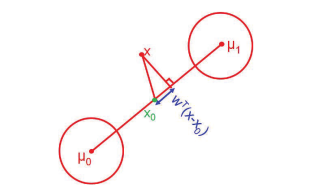
\includegraphics[width=.5\textwidth]{./chaps/32_sec/images/2_geometry_lda.png}
    \end{center}
    \caption{Geometry of LDA in the 2 class case where $\bm{\Sigma}_{1} = \bm{\Sigma}_{0}
= \bm{I}$}
    \label{fig:2_geometry_lda}
\end{figure}





